\documentclass[11pt]{homework}
\usepackage[margin=1in]{geometry}
\usepackage{float}
\fancyheadoffset{0cm}

\newcommand{\hwname}{Luis Pimentel ~~~~~~~~~~~~~~ Jackson Crandell}
\newcommand{\professor}{Professor Evangelos Theodorou}
\newcommand{\hwemail}{lpimentel3@gatech.edu ~~~ jackcrandell@gatech.edu}
\newcommand{\hwtype}{Homework}
\newcommand{\hwnum}{1}
\newcommand{\hwclass}{AE 4803 Robotics and Autonomy}
\newcommand{\hwdate}{October 2, 2020}

\renewcommand{\vec}[1]{\ensuremath{\boldsymbol{#1}}}
\addtolength{\jot}{0.5em}
\allowdisplaybreaks

\usepackage[colorlinks=false]{hyperref}
\usepackage[ruled,vlined]{algorithm2e}

\usepackage{minted}
\usepackage{ dsfont }

\begin{document}
\maketitle

%%%%%%%%%%%%%%%%%%%%%%%%%%%%%%%%%%%%%%%%%%%%%%%%%%%%%%%%%%%%%%%%%%%%%%%%%%%%%%%%%%%%%%% Part 1 
\renewcommand{\questiontype}{Part}
\question

	\begin{arabicparts}
		\questionpart 
			
		First we linearize the dynamics $\frac{d\vec{x}}{dt} = f(\vec{x}, \vec{u}, t)$ :
			
			\begin{align*}
				& \frac{d\vec{x}}{dt} = f(\vec{x}, \vec{u}, t) \\
				& = f(\vec{x} + (\bar{\vec{x}} - \bar{\vec{x}}), \vec{u} + (\bar{\vec{u}} - \bar{\vec{u}}), t) \\
				& = f(\bar{\vec{x}} + (\vec{x} - \bar{\vec{x}}), \bar{\vec{u}} + (\vec{u} - \bar{\vec{u}}), t) \\
				& = f(\bar{\vec{x}} + \delta \vec{x}, \bar{\vec{u}} + \delta \vec{u}, t) \\
				& = f(\bar{\vec{x}}, \bar{\vec{u}}, t) + \nabla_{\vec{x}}f\delta\vec{x} +  \nabla_{\vec{u}}f\delta\vec{u} \\
				& \frac{d\vec{x}}{dt} - f(\bar{\vec{x}}, \bar{\vec{u}}, t) = \nabla_{\vec{x}}f\delta\vec{x} +  \nabla_{\vec{u}}f\delta\vec{u} \\
				& \frac{d\delta\vec{x}}{dt} = \nabla_{\vec{x}}f\delta\vec{x} +  \nabla_{\vec{u}}f\delta\vec{u} 
			\end{align*}
			
		Then we time discretize the linearized dynamics: 
		
			\begin{align*}
				& \frac{\delta \vec{x}(t_{k+1}) - \delta\vec{x}(t_{k})}{t_{k+1} - t_{k}} = \nabla_{\vec{x}}f\delta\vec{x}(t_{k}) +  \nabla_{\vec{u}}f\delta\vec{u}(t_{k}) \\
				& \frac{\delta \vec{x}(t_{k+1}) - \delta\vec{x}(t_{k})}{dt} = \nabla_{\vec{x}}f\delta\vec{x}(t_{k}) +  \nabla_{\vec{u}}f\delta\vec{u}(t_{k}) \\
				& \delta \vec{x}(t_{k+1}) - \delta\vec{x}(t_{k}) = \nabla_{\vec{x}}fdt\delta\vec{x}(t_{k}) +  \nabla_{\vec{u}}fdt\delta\vec{u}(t_{k}) \\
				& \delta \vec{x}(t_{k+1}) = \nabla_{\vec{x}}fdt\delta\vec{x}(t_{k}) + \delta\vec{x}(t_{k}) +  \nabla_{\vec{u}}fdt\delta\vec{u}(t_{k}) \\
				& \delta \vec{x}(t_{k+1}) =  \left(\vec{I}_{n \times n} + \nabla_{\vec{x}}fdt\right)\delta\vec{x}(t_{k}) + (\nabla_{\vec{u}}fdt)\delta\vec{u}(t_{k}) \\
				& \delta \vec{x}(t_{k+1}) =  \vec{\Phi}(t_{k})\delta\vec{x}(t_{k}) + \vec{B}(t_{k})\delta\vec{u}(t_{k}) \\
			\end{align*}
		Where: 
			\begin{align*}
				& \vec{\Phi}(t_{k}) = \vec{I}_{n \times n} + \nabla_{\vec{x}}f(t_{k+1} + t_{k}) \\
				& \vec{B}(t_{k}) = \nabla_{\vec{u}}f(t_{k+1} + t_{k})
			\end{align*}
		
		
		\questionpart
		
		Next we want to express the second-order expansion of $Q(\vec{x}(t_{k}), \vec{u}(t_{k}))$. First we consider the general 2nd Order Taylor Series Expansion of a single-variable function and a multi-variable function:  
			\begin{align*}
				& f(x) \approx f(a) + f'(a)(x-a)^{2} + \frac{f''(a)}{2}(x-a)^{2} at x = a\\
				& f(x,y) \approx f(a,b) + f_{x}(a,b)(x-a) + f_{y}(a,b)(y-b)  \\
				& + \frac{1}{2}f_{xx}(a,b)(x-a)^2 + f_{xy}(a,b)(x-a)(y-b) + \frac{1}{2}f_{yy}(a,b)(y-b)^2 \\
			\end{align*}
		We can generalize these forms in matrix-algebra for our state-action value function.
			\begin{align*}
				& Q(\vec{x}(t_{k}), \vec{u}(t_{k})) = \mathcal{L}(\vec{x}(t_{k}), \vec{u}(t_{k}), t_{k}) + V(\vec{x}(t_{k+1}), t_{k+1})
			\end{align*}
		
		We will start by writing the expansion of the running cost and the value function individually. \\
		
		First we do the second order expansion of the runnning cost along the nominal trajectory $\bar{\vec{x}}$ and $\bar{\vec{u}}$: 
			\begin{align*}
				& \mathcal{L}(\vec{x}(t_{k}), \vec{u}(t_{k}), t_{k}) \\
				& = \mathcal{L}(\vec{x}(t_{k}) + \left(\bar{\vec{x}}(t_{k}) - \bar{\vec{x}}(t_{k})\right), \vec{u}(t_{k}) + \left(\bar{\vec{u}}(t_{k}) - \bar{\vec{u}}(t_{k})\right), t_{k}) \\
				& = \mathcal{L}( \bar{\vec{x}}(t_{k}) + \left(\vec{x}(t_{k}) - \bar{\vec{x}}(t_{k})\right), \bar{\vec{u}}(t_{k}) + \left(\vec{u}(t_{k}) - \bar{\vec{u}}(t_{k})\right), t_{k}) \\
				& = \mathcal{L}(\bar{\vec{x}}(t_{k}) + \delta \vec{x}(t_{k}), \bar{\vec{u}}(t_{k}) + \delta \vec{u}(t_{k}), t_{k}) \\
				& = \underbrace{\ell(\vec{\bar{x}}(t_{k}), \vec{\bar{u}}(t_{k}), t_{k})dt}_{\mathcal{L}} + \underbrace{\Big(\nabla_{\vec{x}}\ell(\vec{x}(t_{k}), \vec{u}(t_{k}), t_{k})dt\Big)^{T}}_{\mathcal{L}_{\vec{x}}}\delta\vec{x}(t_{k}) + \underbrace{\Big(\nabla_{\vec{u}}\ell(\vec{x}(t_{k}), \vec{u}(t_{k}), t_{k})dt\Big)^{T}}_{\mathcal{L}_{\vec{u}}}\delta\vec{u}(t_{k}) \\
				& + \frac{1}{2}\delta\vec{x}(t_{k})^{T}\underbrace{\Big(\nabla_{\vec{xx}}\ell(\vec{x}(t_{k}), \vec{u}(t_{k}), t_{k})dt\Big)}_{\mathcal{L}_{\vec{xx}}}\delta\vec{x}(t_{k}) + \frac{1}{2}\delta\vec{u}(t_{k})^{T}\underbrace{\Big(\nabla_{\vec{uu}}\ell(\vec{x}(t_{k}), \vec{u}(t_{k}), t_{k})dt\Big)}_{\mathcal{L}_{\vec{uu}}}\delta\vec{u}(t_{k}) \\
				& + \frac{1}{2}\delta\vec{u}(t_{k})^{T}\underbrace{\Big(\nabla_{\vec{xu}}\ell(\vec{x}(t_{k}), \vec{u}(t_{k}), t_{k})dt\Big)}_{\mathcal{L}_{\vec{xu}}}\delta\vec{x}(t_{k}) + \frac{1}{2}\delta\vec{x}(t_{k})^{T}\underbrace{\Big(\nabla_{\vec{ux}}\ell(\vec{x}(t_{k}), \vec{u}(t_{k}), t_{k})dt\Big)}_{\mathcal{L}_{\vec{ux}}}\delta\vec{u}(t_{k})\\
			\end{align*}
		\newpage
		We denote:
			\begin{align*}
				& \mathcal{L} = \ell(\vec{\bar{x}}(t_{k}), \vec{\bar{u}}(t_{k}), t_{k})dt \\
				& \mathcal{L}_{\vec{x}} = \nabla_{\vec{x}}\ell(\vec{x}(t_{k}), \vec{u}(t_{k}), t_{k})dt \\
				& \mathcal{L}_{\vec{u}} = \nabla_{\vec{u}}\ell(\vec{x}(t_{k}), \vec{u}(t_{k}), t_{k})dt \\
				& \mathcal{L}_{\vec{xx}} = \nabla_{\vec{xx}}\ell(\vec{x}(t_{k}), \vec{u}(t_{k}), t_{k})dt \\
				& \mathcal{L}_{\vec{uu}} = \nabla_{\vec{uu}}\ell(\vec{x}(t_{k}), \vec{u}(t_{k}), t_{k})dt \\
				& \mathcal{L}_{\vec{xu}} = \nabla_{\vec{xu}}\ell(\vec{x}(t_{k}), \vec{u}(t_{k}), t_{k})dt \\
				& \mathcal{L}_{\vec{ux}} = \nabla_{\vec{ux}}\ell(\vec{x}(t_{k}), \vec{u}(t_{k}), t_{k})dt \\
			\end{align*}
		
		With this we write second order expansion of the running cost as: 
			\begin{align*}
				& \mathcal{L}(\vec{x}(t_{k}), \vec{u}(t_{k}), t_{k}) \\
				& = \mathcal{L} + \mathcal{L}_{\vec{x}}^{T}\delta\vec{x}(t_{k}) + \mathcal{L}_{\vec{u}}^{T}\delta\vec{u}(t_{k}) \\
				& + \frac{1}{2}\delta\vec{x}(t_{k})^{T}\mathcal{L}_{\vec{xx}}\delta\vec{x}(t_{k}) + \frac{1}{2}\delta\vec{u}(t_{k})^{T}\mathcal{L}_{\vec{uu}}\delta\vec{u}(t_{k}) \\
				& + \frac{1}{2}\delta\vec{u}(t_{k})^{T}\mathcal{L}_{\vec{xu}}\delta\vec{x}(t_{k}) + \frac{1}{2}\delta\vec{x}(t_{k})^{T}\mathcal{L}_{\vec{ux}}\delta\vec{u}(t_{k}) \\
			\end{align*} 

		Next we do the second order expansion of the value function along the nominal trajectory $\bar{\vec{x}}$: 
			\begin{align*}
				& V(\vec{x}(t_{k+1}), t_{k+1}) \\
				& = V(\vec{x}(t_{k+1}) + \left(\bar{\vec{x}}(t_{k+1}) - \bar{\vec{x}}(t_{k+1})\right), t_{k+1}) \\
				& = V(\bar{\vec{x}}(t_{k+1}) + \left(\vec{x}(t_{k+1}) - \bar{\vec{x}}(t_{k+1})\right), t_{k+1}) \\
				& = V(\bar{\vec{x}}(t_{k+1}) + \delta\vec{x}(t_{k+1}), t_{k+1}) \\
				& = V(\bar{\vec{x}}(t_{k+1}), t_{k+1}) + \nabla_{\vec{x}}V(\bar{\vec{x}}(t_{k+1}), t_{k+1})^{T}\delta\vec{x}(t_{k+1}) + \frac{1}{2}\delta\vec{x}(t_{k+1})^T\nabla_{\vec{xx}}V(\bar{\vec{x}}(t_{k+1}), t_{k+1})\delta\vec{x}(t_{k+1}) 
			\end{align*}
			
		We denote: 
			\begin{align*}
				& \delta\vec{x}(t_{k+1}) = \vec{x}(t_{k+1}) - \bar{\vec{x}}(t_{k+1}) \\
				& V(t_{k+1}) = V(\bar{\vec{x}}(t_{k+1}), t_{k+1})\\
				& V_{\vec{x}}(t_{k+1}) = \nabla_{\vec{x}}V(\bar{\vec{x}}(t_{k+1}), t_{k+1}) \\
				& V_{\vec{xx}}(t_{k+1}) = \nabla_{\vec{xx}}V(\bar{\vec{x}}(t_{k+1}), t_{k+1})
			\end{align*}
		
		Therefore: 
			\begin{align*}
				&  = V(t_{k+1}) + V_{\vec{x}}(t_{k+1})^{T}\delta\vec{x}(t_{k+1}) + \frac{1}{2}\delta\vec{x}(t_{k+1})^TV_{\vec{xx}}(t_{k+1})\delta\vec{x}(t_{k+1})
			\end{align*}
	
		We recall from the linearized dynamics in Part 1.1 that $\delta \vec{x}(t_{k+1}) =  \vec{\Phi}(t_{k})\delta\vec{x}(t_{k}) + \vec{B}(t_{k})\delta\vec{u}(t_{k})$. Therefore:
		
			\begin{align*}
				&  = V(t_{k+1}) + V_{\vec{x}}(t_{k+1})^{T}\Big(\vec{\Phi}(t_{k})\delta\vec{x}(t_{k}) + \vec{B}(t_{k})\delta\vec{u}(t_{k})\Big) \\
				& + \frac{1}{2}\Big(\vec{\Phi}(t_{k})\delta\vec{x}(t_{k}) + \vec{B}(t_{k})\delta\vec{u}(t_{k})\Big)^TV_{\vec{xx}}(t_{k+1})\Big(\vec{\Phi}(t_{k})\delta\vec{x}(t_{k}) + \vec{B}(t_{k})\delta\vec{u}(t_{k})\Big) \\
				& = V(t_{k+1}) + V_{\vec{x}}(t_{k+1})^{T}\vec{\Phi}(t_{k})\delta\vec{x}(t_{k}) +  V_{\vec{x}}(t_{k+1})^{T}\vec{B}(t_{k})\delta\vec{u}(t_{k}) \\
				& + \frac{1}{2}\delta\vec{x}(t_{k})^{T}\vec{\Phi}(t_{k})^{T}V_{\vec{xx}}(t_{k+1})\vec{\Phi}(t_{k})\delta\vec{x}(t_{k}) + \frac{1}{2}\delta\vec{u}(t_{k})^{T}\vec{B}(t_{k})^{T}V_{\vec{xx}}(t_{k+1})\vec{B}(t_{k})\delta\vec{u}(t_{k}) \\
				& + \frac{1}{2}\delta\vec{u}(t_{k})^{T}\vec{B}(t_{k})^{T}V_{\vec{xx}}(t_{k+1})\vec{\Phi}(t_{k})\delta\vec{x}(t_{k}) + \frac{1}{2}\delta\vec{x}(t_{k})^{T}\vec{\Phi}(t_{k})^{T}V_{\vec{xx}}(t_{k+1})\vec{B}(t_{k})\delta\vec{u}(t_{k})
			\end{align*}
		
		The last two terms can be combined as they evaluate to equal scalars. Therefore, we can simplify the second order expansion of the value function as: 
			\begin{align*}
				& V(\vec{x}(t_{k+1}), t_{k+1}) \\
				& = V(t_{k+1}) + V_{\vec{x}}(t_{k+1})^{T}\vec{\Phi}(t_{k})\delta\vec{x}(t_{k}) +  V_{\vec{x}}(t_{k+1})^{T}\vec{B}(t_{k})\delta\vec{u}(t_{k}) \\
				& + \frac{1}{2}\delta\vec{x}(t_{k})^{T}\vec{\Phi}(t_{k})^{T}V_{\vec{xx}}(t_{k+1})\vec{\Phi}(t_{k})\delta\vec{x}(t_{k}) + \frac{1}{2}\delta\vec{u}(t_{k})^{T}\vec{B}(t_{k})^{T}V_{\vec{xx}}(t_{k+1})\vec{B}(t_{k})\delta\vec{u}(t_{k}) \\
				& + \delta\vec{u}(t_{k})^{T}\vec{B}(t_{k})^{T}V_{\vec{xx}}(t_{k+1})\vec{\Phi}(t_{k})\delta\vec{x}(t_{k}) \\
			\end{align*}
			
		We can now consider the second order expansion of the action-value function itself: 
			\begin{align*}
				& Q(\vec{x}(t_{k}), \vec{u}(t_{k}), t_{k}) \\
				& = Q(\vec{x}(t_{k}) + \left(\bar{\vec{x}}(t_{k}) - \bar{\vec{x}}(t_{k})\right), \vec{u}(t_{k}) + \left(\bar{\vec{u}}(t_{k}) - \bar{\vec{u}}(t_{k})\right), t_{k}) \\
				& = Q( \bar{\vec{x}}(t_{k}) + \left(\vec{x}(t_{k}) - \bar{\vec{x}}(t_{k})\right), \bar{\vec{u}}(t_{k}) + \left(\vec{u}(t_{k}) - \bar{\vec{u}}(t_{k})\right), t_{k}) \\
				& = Q(\bar{\vec{x}}(t_{k}) + \delta \vec{x}(t_{k}), \bar{\vec{u}}(t_{k}) + \delta \vec{u}(t_{k}), t_{k}) \\
				& = Q_{0} + Q_{\vec{x}}^T\delta{\vec{x}}(t_{k}) + Q_{\vec{u}}^T\delta{\vec{u}}(t_{k}) + \frac{1}{2}\delta\vec{x}(t_{k})^{T}Q_{\vec{xx}}\delta\vec{x}(t_{k})  + \frac{1}{2}\delta\vec{u}(t_{k})^{T}Q_{\vec{uu}}\delta\vec{u}(t_{k})\\
				&  + \frac{1}{2}\delta\vec{u}(t_{k})^{T}Q_{\vec{xu}}\delta\vec{x}(t_{k}) + \frac{1}{2}\delta\vec{x}(t_{k})^{T}Q_{\vec{ux}}\delta\vec{u}(t_{k})
			\end{align*}
		Similiarly to the value function expansion, the last two terms can be combined as they evaluate to equal scalars, we can simplify the second order expansion of the state-action value function as:
			\begin{align*}
				& Q(\bar{\vec{x}}(t_{k}) + \delta \vec{x}(t_{k}), \bar{\vec{u}}(t_{k}) + \delta \vec{u}(t_{k}), t_{k}) \\
				& = Q_{0} + Q_{\vec{x}}^T\delta{\vec{x}}(t_{k}) + Q_{\vec{u}}^T\delta{\vec{u}}(t_{k}) + \frac{1}{2}\delta\vec{x}(t_{k})^{T}Q_{\vec{xx}}\delta\vec{x}(t_{k})  + \frac{1}{2}\delta\vec{u}(t_{k})^{T}Q_{\vec{uu}}\delta\vec{u}(t_{k})\\
				& + \delta\vec{x}(t_{k})^{T}Q_{\vec{ux}}\delta\vec{u}(t_{k})
			\end{align*}
			
			
			\newpage 
		Finally we can combine the second order expansions of the running cost and value function to express the second order expansion of the state-action value function: 
			\begin{align*}
				& Q(\bar{\vec{x}}(t_{k}) + \delta \vec{x}(t_{k}), \bar{\vec{u}}(t_{k}) + \delta \vec{u}(t_{k}), t_{k}) \\
				& = \mathcal{L} + \mathcal{L}_{\vec{x}}^{T}\delta\vec{x}(t_{k}) + \mathcal{L}_{\vec{u}}^{T}\delta\vec{u}(t_{k}) + \frac{1}{2}\delta\vec{x}(t_{k})^{T}\mathcal{L}_{\vec{xx}}\delta\vec{x}(t_{k}) + \frac{1}{2}\delta\vec{u}(t_{k})^{T}\mathcal{L}_{\vec{uu}}\delta\vec{u}(t_{k}) \\
				& + \frac{1}{2}\delta\vec{u}(t_{k})^{T}\mathcal{L}_{\vec{xu}}\delta\vec{x}(t_{k}) + \frac{1}{2}\delta\vec{x}(t_{k})^{T}\mathcal{L}_{\vec{ux}}\delta\vec{u}(t_{k}) \\
				& + V(t_{k+1}) + V_{\vec{x}}(t_{k+1})^{T}\vec{\Phi}(t_{k})\delta\vec{x}(t_{k}) +  V_{\vec{x}}(t_{k+1})^{T}\vec{B}(t_{k})\delta\vec{u}(t_{k}) \\
				& + \frac{1}{2}\delta\vec{x}(t_{k})^{T}\vec{\Phi}(t_{k})^{T}V_{\vec{xx}}(t_{k+1})\vec{\Phi}(t_{k})\delta\vec{x}(t_{k}) + \frac{1}{2}\delta\vec{u}(t_{k})^{T}\vec{B}(t_{k})^{T}V_{\vec{xx}}(t_{k+1})\vec{B}(t_{k})\delta\vec{u}(t_{k}) \\
				& + \delta\vec{u}(t_{k})^{T}\vec{B}(t_{k})^{T}V_{\vec{xx}}(t_{k+1})\vec{\Phi}(t_{k})\delta\vec{x}(t_{k})
			\end{align*}
	
		We can group the zero, first, and second order terms as: 
			\begin{align*}
				& = \underbrace{\Big(\mathcal{L} +  V(t_{k+1})  \Big)}_{Q_{0}} + \underbrace{\Big(\mathcal{L}_{\vec{x}} + \vec{\Phi}(t_{k})^{T}V_{\vec{x}}(t_{k+1}) \Big)^{T}}_{Q_{\vec{x}}}\delta\vec{x}(t_{k})  + \underbrace{\Big(\mathcal{L}_{\vec{u}} + \vec{B}(t_{k})^{T}V_{\vec{x}}(t_{k+1})\Big)^{T}}_{Q_{\vec{u}}}\delta\vec{u}(t_{k}) \\
				& + \frac{1}{2}\delta\vec{x}(t_{k})^{T}\underbrace{\Big( \mathcal{L}_{\vec{xx}} + \vec{\Phi}(t_{k})^{T}V_{\vec{xx}}(t_{k+1})\vec{\Phi}(t_{k})\Big)}_{Q_{\vec{xx}}}\delta\vec{x}(t_{k}) \\
				& + \frac{1}{2}\delta\vec{u}(t_{k})^{T}\underbrace{\Big(\mathcal{L}_{\vec{uu}} + \vec{B}(t_{k})^{T}V_{\vec{xx}}(t_{k+1})\vec{B}(t_{k})\Big)}_{Q_{\vec{uu}}}\delta\vec{u}(t_{k}) \\
				& + \delta\vec{u}(t_{k})^{T}\underbrace{\Bigg( \frac{1}{2}\mathcal{L}_{\vec{ux}} + \frac{1}{2}\mathcal{L}_{\vec{xu}}^{T} + \frac{1}{2}\vec{B}(t_{k})^{T}\Big(V_{\vec{xx}}(t_{k+1}) + V_{\vec{xx}}(t_{k+1})^{T}\Big) \vec{\Phi}(t_{k})\Bigg)}_{Q_{\vec{ux}}}\delta\vec{x}(t_{k})
			\end{align*}
		
		Where we denote: 
		\begin{align*}
			& Q_{0} = \mathcal{L} +  V(t_{k+1})  \\
			& Q_{\vec{x}} = \mathcal{L}_{\vec{x}} + \vec{\Phi}(t_{k})^{T}V_{\vec{x}}(t_{k+1}) \\
			& Q_{\vec{u}} = \mathcal{L}_{\vec{u}} + \vec{B}(t_{k})^{T}V_{\vec{x}}(t_{k+1}) \\
			& Q_{\vec{xx}} = \mathcal{L}_{\vec{xx}} + \vec{\Phi}(t_{k})^{T}V_{\vec{xx}}(t_{k+1})\vec{\Phi}(t_{k}) \\
			& Q_{\vec{uu}} = \mathcal{L}_{\vec{uu}} + \vec{B}(t_{k})^{T}V_{\vec{xx}}(t_{k+1})\vec{B}(t_{k}) \\
			& Q_{\vec{ux}} = \vec{B}(t_{k})^{T}V_{\vec{xx}}(t_{k+1})\vec{\Phi}(t_{k}) + \mathcal{L}_{\vec{ux}}
		\end{align*}
	
	\newpage
		\questionpart
		
	
		Next we compute the optimal control corrections $\delta\vec{u}^{*}(t_{k})$. We do this by minimizing $\delta\vec{u}(t_{k})$ with respect to the state-action value function $Q(\vec{x}(t_{k}), \vec{u}(t_{k}))$. This is the same as minimizing $\vec{u}(t_{k})$ to compute the locally optimal control $\vec{u}^{*}(t_{k})$ in the Bellman Principle. This so since $\vec{u}^{*}(t_{k}) = \bar{\vec{u}}(t_{k}) + \delta\vec{u}^{*}(t_{k})$. 

			\begin{align*}
				& \underset{\delta\vec{u}(t_{k})}{\text{min}} ~ \Bigg[ Q(\vec{x}(t_{k}), \vec{u}(t_{k})) \Bigg] \\
				& = \underset{\delta\vec{u}(t_{k})}{\text{min}} ~ \Bigg[ \Big(\mathcal{L} +  V(t_{k+1})  \Big) + \Big(\mathcal{L}_{\vec{x}} + \vec{\Phi}(t_{k})^{T}V_{\vec{x}}(t_{k+1}) \Big)^{T}\delta\vec{x}(t_{k})  + \Big(\mathcal{L}_{\vec{u}} + \vec{B}(t_{k})^{T}V_{\vec{x}}(t_{k+1})\Big)^{T}\delta\vec{u}(t_{k}) \\
				& + \frac{1}{2}\delta\vec{x}(t_{k})^{T}\Big( \mathcal{L}_{\vec{xx}} + \vec{\Phi}(t_{k})^{T}V_{\vec{xx}}(t_{k+1})\vec{\Phi}(t_{k})\Big)\delta\vec{x}(t_{k}) + \frac{1}{2}\delta\vec{u}(t_{k})^{T}\Big( \mathcal{L}_{\vec{uu}} + \vec{B}(t_{k})^{T}V_{\vec{xx}}(t_{k+1})\vec{B}(t_{k})\Big)\delta\vec{u}(t_{k}) \\
				& + \delta\vec{u}(t_{k})^{T}\Bigg( \frac{1}{2}\mathcal{L}_{\vec{ux}} + \frac{1}{2}\mathcal{L}_{\vec{xu}}^{T} + \frac{1}{2}\vec{B}(t_{k})^{T}\Big(V_{\vec{xx}}(t_{k+1}) + V_{\vec{xx}}(t_{k+1})^{T}\Big) \vec{\Phi}(t_{k})\Bigg)\delta\vec{x}(t_{k})\Bigg]
			\end{align*}
			
			
		To solve this take the gradient of $Q(\vec{x}(t_{k}), \vec{u}(t_{k}))$ with respect to $\delta\vec{u}(t_{k})$ and set it equal to zero:
			\begin{align*}
				& 0 = \underbrace{\Big(\mathcal{L}_{\vec{u}} + \vec{B}(t_{k})^{T}V_{\vec{x}}(t_{k+1})\Big)}_{Q_{\vec{u}}} +  \underbrace{\Bigg( \frac{1}{2}\mathcal{L}_{\vec{ux}} + \frac{1}{2}\mathcal{L}_{\vec{xu}}^{T} + \frac{1}{2}\vec{B}(t_{k})^{T}\Big(V_{\vec{xx}}(t_{k+1}) + V_{\vec{xx}}(t_{k+1})^{T}\Big) \vec{\Phi}(t_{k})  \Bigg)}_{Q_{\vec{ux}}}\delta\vec{x}(t_{k}) \\
				& + \underbrace{\Big( \mathcal{L}_{\vec{uu}} + \vec{B}(t_{k})^{T}V_{\vec{xx}}(t_{k+1})\vec{B}(t_{k})\Big)}_{Q_{\vec{uu}}}\delta\vec{u}(t_{k}) \\
			\end{align*}
	
		Therefore: 
			\begin{align*}
				& 0 = Q_{\vec{u}} + Q_{\vec{ux}}\delta\vec{x}(t_{k})  + Q_{\vec{uu}}\delta\vec{u}(t_{k}) \\
				& -Q_{\vec{uu}}\delta\vec{u}(t_{k}) = Q_{\vec{u}} + Q_{\vec{ux}}\delta\vec{x}(t_{k})  \\
				& \delta\vec{u}(t_{k}) = \underbrace{-Q_{\vec{uu}}^{-1}Q_{\vec{u}}}_{\vec{l}_{\vec{u}}(t_{k})} + \underbrace{\Big(-Q_{\vec{uu}}^{-1} Q_{\vec{ux}}\Big)}_{\vec{L}_{\vec{u}}(t_{k})}\delta\vec{x}(t_{k}) 
			\end{align*}
		Further, we denote $\vec{l}_{\vec{u}}(t_{k})$ as the feedforward term and $\vec{L}_{\vec{u}}(t_{k})$ as the feedback term: 
			\begin{align*}
				& \vec{l}_{\vec{u}}(t_{k}) = -Q_{\vec{uu}}^{-1}Q_{\vec{u}} \\
				& \vec{L}_{\vec{u}}(t_{k}) = -Q_{\vec{uu}}^{-1}Q_{\vec{ux}}
			\end{align*}
		
		And determine  the optimal control corrections to be: 
			\begin{align*}
				& \delta\vec{u}^{*}(t_{k}) = \vec{l}_{\vec{u}}(t_{k}) + \vec{L}_{\vec{u}}(t_{k})\delta\vec{x}(t_{k})\\
			\end{align*}


		\questionpart
	We can compute the equations $V(t_k), V_{\vec{x}}(t_k), V_{\vec{xx}}(t_k)$ in backward time by substituting in our optimal control correction $\delta\vec{u}^{*}(t_{k})$ into the expanded state-action value function $Q(\vec{x}(t_{k}), \vec{u}(t_{k}))$. 
			\begin{align*}
				& Q(\vec{x}(t_{k}), \vec{u}(t_{k}))\Big|_{\delta\vec{u}^{*}(t_{k}) = \vec{l}_{\vec{u}}(t_{k}) + \vec{L}_{\vec{u}}(t_{k})\delta\vec{x}(t_{k})} \\
				& =  Q_{0} + Q_{\vec{x}}^{T}\delta\vec{x}(t_{k}) + Q_{\vec{u}}^{T}\Big(\vec{l}_{\vec{u}}(t_{k}) + \vec{L}_{\vec{u}}(t_{k})\delta\vec{x}(t_{k})\Big) \\
				& + \frac{1}{2}\delta\vec{x}(t_{k})^{T}Q_{\vec{xx}}\delta\vec{x}(t_{k}) + \frac{1}{2}\Big(\vec{l}_{\vec{u}}(t_{k}) + \vec{L}_{\vec{u}}(t_{k})\delta\vec{x}(t_{k})\Big)^{T}Q_{\vec{uu}}\Big(\vec{l}_{\vec{u}}(t_{k}) + \vec{L}_{\vec{u}}(t_{k})\delta\vec{x}(t_{k})\Big) \\
				& + \frac{1}{2}\Big(\vec{l}_{\vec{u}}(t_{k}) + \vec{L}_{\vec{u}}(t_{k})\delta\vec{x}(t_{k})\Big)^{T}Q_{\vec{ux}}\delta\vec{x}(t_{k}) + \frac{1}{2}\delta\vec{x}(t_{k})^{T}Q_{\vec{xu}}\Big(\vec{l}_{\vec{u}}(t_{k}) + \vec{L}_{\vec{u}}(t_{k})\delta\vec{x}(t_{k})\Big) \\
			\end{align*}
		To compute the backward terms we can denote:
			\begin{align*}
				& V(\bar{\vec{x}}(t_{k}) + \delta\vec{x}(t_{k}),t) = V(t_k) + V_{\vec{x}}(t_{k})^T\delta\vec{x}(t_{k}) + \frac{1}{2}\delta\vec{x}(t_{k})^TV_{\vec{xx}}(t_{k})\delta\vec{x}(t_{k}) 
			\end{align*}

		Therefore the zero order terms of the state-action value function in $\delta\vec{x}$ are equal to $V(t_k)$, the first order terms are equal to $V_{\vec{x}}(t_{k})$, and the second order terms are equal to $V_{\vec{xx}}(t_{k})$. \\
	
		First can group the zero order terms that equate to $V(t_k)$: 
			\begin{align*}
				& V(t_k) = Q_{0} + Q_{\vec{u}}^{T}\vec{l}_{\vec{u}}(t_{k}) + \frac{1}{2}\vec{l}_{\vec{u}}(t_{k})^{T}Q_{\vec{uu}}\vec{l}_{\vec{u}}(t_{k})
			\end{align*}
		Next we can group the first order terms that equate to $V_{\vec{x}}(t_{k})$:
			\begin{align*}
				& V_{\vec{x}}(t_{k}) = Q_{\vec{x}} + Q_{\vec{u}}^{T}\vec{L}_{\vec{u}}(t_{k}) + Q_{\vec{xu}}\vec{l}_{\vec{u}}(t_{k}) + \vec{L}_{\vec{u}}(t_{k})^{T}Q_{\vec{uu}}\vec{l}_{\vec{u}}(t_{k}) 
			\end{align*}
		Finally we can group the first order terms that equate to $V_{\vec{xx}}(t_{k})$:
			\begin{align*}
				& V_{\vec{xx}}(t_{k}) = Q_{\vec{xx}} + \vec{L}_{\vec{u}}(t_{k})^{T}Q_{\vec{uu}}\vec{L}_{\vec{u}}(t_{k}) + \vec{L}_{\vec{u}}(t_{k})^{T}Q_{\vec{ux}} + Q_{\vec{xu}}\vec{L}_{\vec{u}}(t_{k}) 
			\end{align*}
	
		In summary, the backward equations can be expressed as: 
			\begin{align*}
				& V(t_k) = Q_{0} + Q_{\vec{u}}^{T}\vec{l}_{\vec{u}}(t_{k}) + \frac{1}{2}\vec{l}_{\vec{u}}(t_{k})^{T}Q_{\vec{uu}}\vec{l}_{\vec{u}}(t_{k}) \\
				& V_{\vec{x}}(t_{k}) = Q_{\vec{x}} + Q_{\vec{u}}^{T}\vec{L}_{\vec{u}}(t_{k}) + Q_{\vec{xu}}\vec{l}_{\vec{u}}(t_{k}) + \vec{L}_{\vec{u}}(t_{k})^{T}Q_{\vec{uu}}\vec{l}_{\vec{u}}(t_{k}) \\
				& V_{\vec{xx}}(t_{k}) = Q_{\vec{xx}} + \vec{L}_{\vec{u}}(t_{k})^{T}Q_{\vec{uu}}\vec{L}_{\vec{u}}(t_{k}) + \vec{L}_{\vec{u}}(t_{k})^{T}Q_{\vec{ux}} + Q_{\vec{xu}}\vec{L}_{\vec{u}}(t_{k})  \\
			\end{align*}
			
		\newpage
		Further we can express these simply as functions of state-action value function by substituting in $\vec{l}_{\vec{u}}(t_{k})$ and $\vec{L}_{\vec{u}}(t_{k})$ : \\
		
		We do this for the value function: 
			\begin{align*}
				& V(t_k) = Q_{0} + Q_{\vec{u}}^{T}\Big(-Q_{\vec{uu}}^{-1}Q_{\vec{u}}\Big) + \frac{1}{2}\Big(-Q_{\vec{uu}}^{-1}Q_{\vec{u}}\Big)^{T}Q_{\vec{uu}}\Big(-Q_{\vec{uu}}^{-1}Q_{\vec{u}}\Big) \\
				& = Q_{0} - Q_{\vec{u}}^{T}Q_{\vec{uu}}^{-1}Q_{\vec{u}} + \frac{1}{2}Q_{\vec{u}}^{T}Q_{\vec{uu}}^{-1}\underbrace{Q_{\vec{uu}}Q_{\vec{uu}}^{-1}}_{\vec{I}}Q_{\vec{u}} \\
				& = Q_{0} - Q_{\vec{u}}^{T}Q_{\vec{uu}}^{-1}Q_{\vec{u}} + \frac{1}{2}Q_{\vec{u}}^{T}Q_{\vec{uu}}^{-1}Q_{\vec{u}} \\
				& = Q_{0} - \frac{1}{2}Q_{\vec{u}}^{T}Q_{\vec{uu}}^{-1}Q_{\vec{u}} 
			\end{align*}
			
		Then, we do this for the gradient of the value function: 
			\begin{align*}
				& V_{\vec{x}}(t_{k}) = Q_{\vec{x}} + Q_{\vec{u}}^{T}\Big(-Q_{\vec{uu}}^{-1}Q_{\vec{ux}}\Big) + Q_{\vec{xu}}\Big(-Q_{\vec{uu}}^{-1}Q_{\vec{u}} \Big)+ \Big(-Q_{\vec{uu}}^{-1}Q_{\vec{ux}}\Big)^{T}Q_{\vec{uu}}\Big(-Q_{\vec{uu}}^{-1}Q_{\vec{u}}\Big) \\
				& = Q_{\vec{x}} - Q_{\vec{u}}^{T}Q_{\vec{uu}}^{-1}Q_{\vec{ux}} - Q_{\vec{xu}}Q_{\vec{uu}}^{-1}Q_{\vec{u}} + Q_{\vec{ux}}^{T}Q_{\vec{uu}}^{-1}\underbrace{Q_{\vec{uu}}Q_{\vec{uu}}^{-1}}_{\vec{I}}Q_{\vec{u}} \\
				& = Q_{\vec{x}} - Q_{\vec{u}}^{T}Q_{\vec{uu}}^{-1}Q_{\vec{ux}} - Q_{\vec{xu}}Q_{\vec{uu}}^{-1}Q_{\vec{u}} + Q_{\vec{u}}^{T}Q_{\vec{uu}}^{-1}Q_{\vec{ux}} \\
				& = Q_{\vec{x}} - Q_{\vec{xu}}Q_{\vec{uu}}^{-1}Q_{\vec{u}} 
			\end{align*}
		
		Finally, we do this for the Hessian of the value function: 
			\begin{align*}
				& V_{\vec{xx}}(t_{k}) = Q_{\vec{xx}} + \vec{L}_{\vec{u}}(t_{k})^{T}Q_{\vec{uu}}\vec{L}_{\vec{u}}(t_{k}) + \vec{L}_{\vec{u}}(t_{k})^{T}Q_{\vec{ux}} + Q_{\vec{xu}}\vec{L}_{\vec{u}}(t_{k})  \\
				& = Q_{\vec{xx}} + \Big(-Q_{\vec{uu}}^{-1}Q_{\vec{ux}} \Big)^{T}Q_{\vec{uu}}\Big(-Q_{\vec{uu}}^{-1}Q_{\vec{ux}} \Big) + \Big(-Q_{\vec{uu}}^{-1}Q_{\vec{ux}} \Big)^{T}Q_{\vec{ux}} + Q_{\vec{xu}}\Big(-Q_{\vec{uu}}^{-1}Q_{\vec{ux}} \Big) \\
				& = Q_{\vec{xx}} + Q_{\vec{ux}}^{T}Q_{\vec{uu}}^{-1}\underbrace{Q_{\vec{uu}}Q_{\vec{uu}}^{-1}}_{\vec{I}}Q_{\vec{ux}}  - Q_{\vec{ux}}^{T}Q_{\vec{uu}}^{-1}Q_{\vec{ux}} - Q_{\vec{xu}}Q_{\vec{uu}}^{-1}Q_{\vec{ux}} \\
				& = Q_{\vec{xx}} + Q_{\vec{ux}}^{T}Q_{\vec{uu}}^{-1}Q_{\vec{ux}}  - Q_{\vec{ux}}^{T}Q_{\vec{uu}}^{-1}Q_{\vec{ux}} - Q_{\vec{xu}}Q_{\vec{uu}}^{-1}Q_{\vec{ux}} \\
				& = Q_{\vec{xx}} - Q_{\vec{xu}}Q_{\vec{uu}}^{-1}Q_{\vec{ux}}\\
			\end{align*}		
		
	\end{arabicparts}

		In summary, the backward equations can be expressed as functions of the state-action value function as: 

			\begin{align*}
				& V(t_k) = Q_{0} - \frac{1}{2}Q_{\vec{u}}^{T}Q_{\vec{uu}}^{-1}Q_{\vec{u}} \\
				& V_{\vec{x}}(t_{k}) = Q_{\vec{x}} - Q_{\vec{xu}}Q_{\vec{uu}}^{-1}Q_{\vec{u}} \\
				& V_{\vec{xx}}(t_{k}) = Q_{\vec{xx}} - Q_{\vec{xu}}Q_{\vec{uu}}^{-1}Q_{\vec{ux}} \\
			\end{align*}

	\newpage

%%%%%%%%%%%%%%%%%%%%%%%%%%%%%%%%%%%%%%%%%%%%%%%%%%%%%%%%%%%%%%%%%%%%%%%%%%%%%%%%%%%%%%% Part 3 
\setcounter{questionCounter}{1}
\renewcommand{\questiontype}{Part}
\question
\begin{arabicparts}
%\setcounter{questionCounter}{2}


\questionpart
See MATLAB code implementation.

\questionpart
See MATLAB code implementation.

\questionpart

	In this problem we are asked to test the robustness of our DDP policy against stochastic forces that act as disturbances in our dynamics. 
		\begin{align*}
			& I\ddot{\theta} + b\dot{\theta} + mglsin(\theta) = u + f_{stochastic}
		\end{align*}
	
	We do this by running the DDP optimization until it converges. This results in an optimal trajectory $\vec{x}^{*}(t_{k})$, optimal control input $\vec{u}^{*}(t_{k})$, and optimal feeback gains $\vec{L}^{*}(t_{k})$. 
	We then initialize a new trajectory and propagate the dynamics forward using the following controller: $\vec{u}(t_{k}) = \vec{u}^{*}(t_{k}) + \vec{L}^{*}(t_{k})\big(\vec{x}(t_{k}) - \vec{x}^{*}(t_{k}) \big)$ \\
	
	This process is repeated for many trajectories throught the following algorithm:
	
	\begin{algorithm}[H]
		\SetAlgoLined
 		initialize: $\vec{x}^{*}(t_{k}), \vec{u}^{*}(t_{k}), \vec{L}^{*}(t_{k})$\;
 		initialize: $ \vec{H}$: time horizon, $dt$ :time step, $ \vec{num\_traj}$: number of trajectories\;
 		initialize: $\vec{F_{x}}(\vec{x}(t_{k})), \vec{F_{u}}(\vec{u}(t_{k}))$: dynamics\;
 		initialize: $\vec{x}(t_{k}) = \vec{0}$\;
 		initialize: $\sigma$: noise level\;
 		
 		\For{$\vec{i} = 1$ to $\vec{num\_traj}$}{
  			\For{$\vec{k} = 1$ to $\vec{H} - 1$}{
  				$R = $ randn\;
  				$\vec{u}(t_{k}) = \vec{u}^{*}(t_{k}) + \vec{L}^{*}(t_{k})\big(\vec{x}(t_{k}) - \vec{x}^{*}(t_{k}) \big)$\;
  				$\vec{x}(t_{k+1}) = \vec{F_{x}}(\vec{x}(t_{k}))dt + \vec{F_{u}}(\vec{u}(t_{k}))dt + \vec{F_{u}}(\vec{u}(t_{k}))R\sigma\sqrt{dt}$
  			}
 		}
 		\caption{DDP Robustness Test Against Stochastic Forces}
	\end{algorithm}
	\newpage
	The following plot shows the results of DDP after optimization:
	
		\begin{figure}[H]
			\centering
			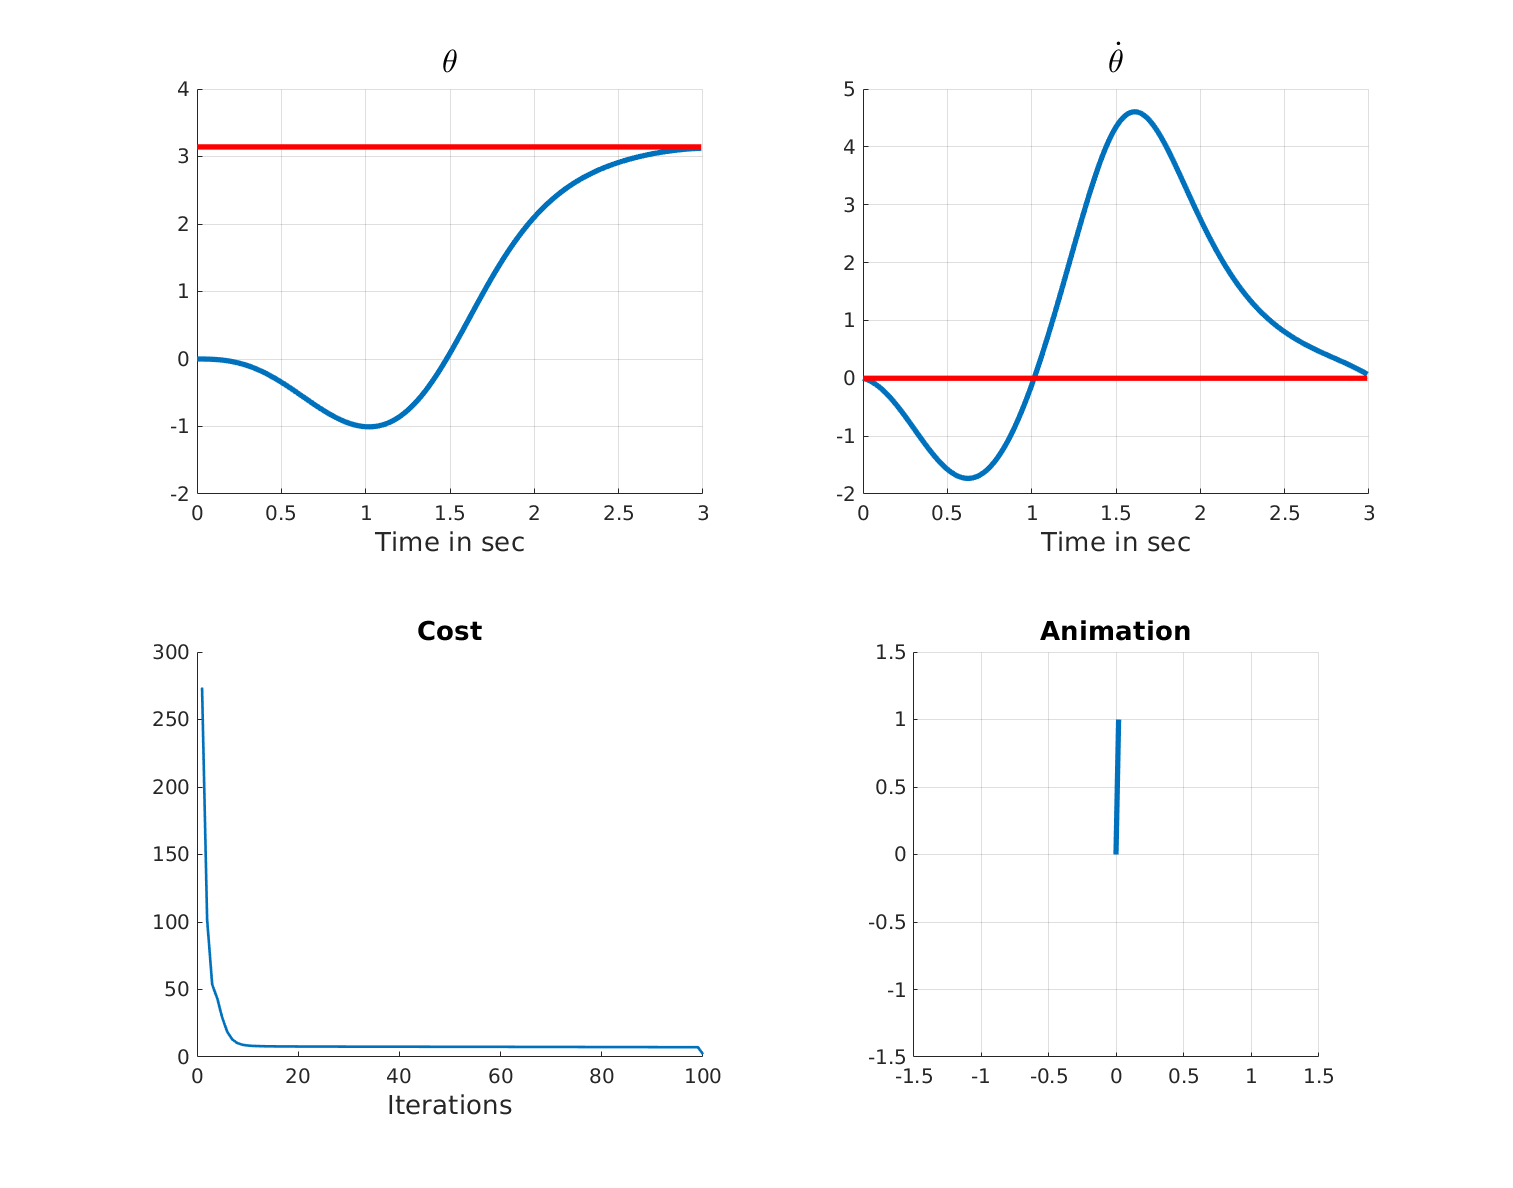
\includegraphics[scale=0.13]{clean_results.png}
			\caption{DDP optimal results.}
		\end{figure}
		
	The following plot shows the results of running the Robustness Test algorithm for 20 trajectories using the optimal DDP trajectory, controller, and feedback gains:
	
		\begin{figure}[H]
			\centering
			\includegraphics[scale=0.16]{robust_test.png}
			\caption{Robustness Test results.}
		\end{figure}

\end{arabicparts}

	






\end{document}
